\section{Tensor completion}
\label{sec:tensor-completion}


Tensor data, which can be viewed as a higher-order generalization of matrix data,  are routinely used in science and engineering applications to capture multi-way interactions across variables of interest \citep{kolda2009tensor,sidiropoulos2017tensor,anandkumar2014tensor}. Akin to matrix completion,   the problem of tensor completion aims to  reconstruct a (structured) tensor when the vast majority of its entries are unobserved, a task that spans a wide spectrum of applications including  visual data inpainting, harmonic retrieval,  seismic data analysis, and so on \citep{liu2012tensor,chen2013spectral,kreimer2013tensor}.


Apparently, this task cannot possibly be accomplished without exploiting further structural assumptions on the tensor under consideration. Inspired by the success of low-rank matrix completion, we explore the case where the unknown tensor enjoys certain low-rank structure (more specifically, low canonical-polyadic (CP) rank~\citep{kolda2009tensor}). For simplicity, we concentrate on order-three tensors (namely, $\bm{T}=[T_{i,j,k}]\in \mathbb{R}^{n_1\times n_2\times n_3}$), which already capture several fundamental challenges intrinsic to tensor estimation. In addition, we take the dimensionality $n_1 = n_2 = n_3 = n$ for simplicity of presentation.




\begin{figure}
\begin{center}
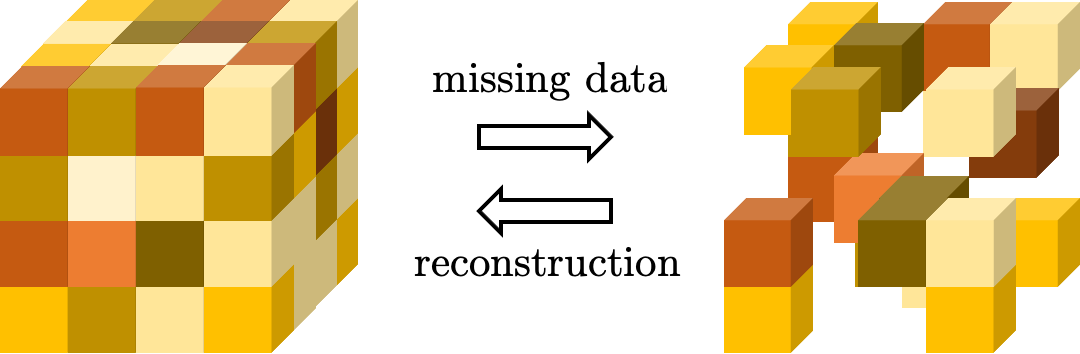
\includegraphics[width=0.65\textwidth]{figures/tensor_completion_plot.png}
\end{center}
\caption{Illustration of tensor completion, where we observe partial entries of an order-three tensor.\label{fig:tensor-completion-illustration}}
\end{figure}





\subsection{Problem formulation and assumptions}
\label{sec:setup-tensor-completion}


\paragraph{Notation.} Before describing our models, we introduce several notation that will be useful throughout. For any vectors $\bm{a}=[a_{i}]_{1\leq i\leq n},\bm{b}=[b_{i}]_{1\leq i\leq n},\bm{c}=[c_{i}]_{1\leq i\leq n}\in\mathbb{R}^{n}$,
the tensor $\bm{a}\otimes\bm{b}\otimes\bm{c}$ stands for an $n\times n\times n$
array whose $(i,j,k)$-th entry is given by $a_{i}b_{j}c_{k}$. Additionally, we denote by $\bm{a}\otimes \bm{b}\coloneqq  {\scriptsize \left[\begin{array}{c}
a_{1}\bm{b}\\
\vdots\\
a_{n}\bm{b}
\end{array}\right]}$ the Kronecker product between $\bm{a}$ and $\bm{b}$.  For any tensor $\bm{T}=[T_{i,j,k}]_{1\leq i,j,k\leq n}\in \mathbb{R}^{n\times n\times n}$, we say that $\bm{A}=[A_{i,j}]\in \mathbb{R}^{n\times n^2}$ is the mode-1 matricization of $\bm{T}$, denoted by $$\bm{A}=\mathsf{unfold}(\bm{T}),$$  if $A_{i,(j-1)n+k} = T_{i,j,k}$ for all $(i,j,k)\in [n]\times [n] \times [n]$.



\paragraph{Models and assumptions.}
Suppose the unknown order-three symmetric tensor $\bm{T}^{\star}=[T_{i,j,k}^{\star}]_{1\leq i,j,k\leq n}$  is a superposition of $r$ ($r<n$) rank-one symmetric tensors:
%
\begin{equation}
\bm{T}^{\star}=\sum_{i=1}^{r}\bm{w}_{i}^{\star}\otimes\bm{w}_{i}^{\star}\otimes\bm{w}_{i}^{\star} \in \mathbb{R}^{n\times n\times n},
\label{eq:defn-true-tensor}
\end{equation}
%
where $\{\bm{w}_i^{\star}\in \mathbb{R}^{n}\}$ represents a set of latent tensor factors.
What we have available are incomplete observations of the entries of  $\bm{T}^{\star}$. The observed data can be succinctly encoded by an index subset $\Omega \subseteq [n]\times [n] \times [n]$ (called a sampling set) and a tensor $\bm{T}=[T_{i,j,k}]_{1\leq i,j,k\leq n}$ as follows
%
\begin{equation}
T_{i,j,k}=\begin{cases}
T_{i,j,k}^{\star},\qquad & \text{if }(i,j,k)\in\Omega,\\
0, & \text{else}.
\end{cases}
\label{eq:observed-tensor-T}
\end{equation}
%
This subsection aims for an intermediate goal, namely, estimating the subspace spanned by $\{\bm{w}_i^{\star}\}_{1\leq i\leq r}$, which often serves as a crucial initial stage towards reliable completion of the whole tensor. The interested reader is referred to \citet{montanari2016spectral,cai2019tensorOR} for subsequent stages of tensor completion algorithms.


Similar to the matrix completion counterpart, we explore a {\em random sampling} pattern such that for all $(i,j,k)\in [n]\times [n] \times [n]$,
%
\begin{align}
	(i,j,k) \in \Omega \qquad \text{independently with probability }p.
\end{align}
%
In addition, we define for notational convenience that
%
\begin{equation}
	\nu_{i}\coloneqq\|\bm{w}_{i}^{\star}\|_{2}^{3},\qquad \nu_{\min}\coloneqq \min_{1\leq i\leq r}\nu_{i},\qquad \nu_{\max} \coloneqq \max_{1\leq i\leq r}\nu_{i},
	\label{eq:defn-wi-wmin-wmax-TC}
\end{equation}
%
where $\nu_{i}$ reflects the size of the rank-1 component $\bm{w}_{i}^{\star}\otimes \bm{w}_{i}^{\star}\otimes \bm{w}_{i}^{\star}$. The condition number of $\bm{T}^{\star}$ is then defined as $\kappa \coloneqq \nu_{\max} / \nu_{\min}$.

We shall also introduce several incoherence parameters as follows.
%
\begin{definition}
	Define the incoherence parameters of $\bm{T}^{\star}$ (cf.~\eqref{eq:defn-true-tensor}) as
	%
	\begin{equation}
		\mu_{1}\coloneqq\max_{1\leq i\leq r}\frac{n\|\bm{w}_{i}^{\star}\|_{\infty}^{2}}{\|\bm{w}_{i}^{\star}\|_{2}^{2}},
		\quad \text{and} \quad
		\mu_{2}\coloneqq\max_{i\neq j}\frac{n\big|\langle\bm{w}_{i}^{\star},\bm{w}_{j}^{\star}\rangle\big|^{2}}{\|\bm{w}_{i}^{\star}\|_{2}^{2} \, \|\bm{w}_{j}^{\star}\|_{2}^{2}} .
		\label{eq:defn-incoherence-TC}
	\end{equation}
	%
\end{definition}
%
Let us explain these parameters in words: small $\mu_1$ and $\mu_2$ reflect that (i) the energy of each tensor factor $\bm{w}_i^{\star}$ is spread out across different entries, and (ii) the factors $\{\bm{w}_i^{\star}\}$  are not too correlated with each other. To simplify presentation, we set
%
\begin{align*}
	\mu \coloneqq \max \{ \mu_1, \mu_2 \}.
\end{align*}


\subsection{Algorithm}
\label{sec:algorithm-TC}


Unfortunately, it is notoriously difficult to exploit the low-rank structure---and many other low-complexity structure---efficiently in the original tensor space \citep{hillar2013most}.
To circumvent this issue,
a natural strategy thus attempts to matricize the tensor data, followed by an application of suitable low-rank matrix estimation algorithms.   Specifically, let us unfold the tensor $\bm{T}^{\star}$ into an $n\times n^2$ matrix $\bm{A}^{\star}$ as follows
%
\begin{align}
	\bm{A}^{\star}\coloneqq \mathsf{unfold}\big( \bm{T}^{\star}\big)
	= \sum_{i=1}^{r}\bm{w}_{i}^{\star}\big(\bm{w}_{i}^{\star}\otimes\bm{w}_{i}^{\star}\big)^{\top} \in \mathbb{R}^{n\times n^2}.
	\label{eq:defn-Astar-TC}	
\end{align}
%
The resulting matrix $\bm{A}^{\star}$ inherits the low-rank structure, as it clearly has rank at most $r$. We shall also matricize the observed data as
%
\begin{align}
	\bm{A} \coloneqq \mathsf{unfold} ( \bm{T} ) .
	\label{eq:defn-A-TC}
\end{align}


In order to estimate the subspace $\bm{U}^{\star}$ spanned by $\{\bm{w}_i^{\star}\}_{1\leq i\leq r}$ (which is  the column space of $\bm{A}^{\star}$ as well), the spectral method studied here resorts to the rescaled Gram matrix $p^{-2} \bm{A} \bm{A}^{\top}$. As a sanity check, if there is absolutely no missing data (i.e., $p=1$), then $p^{-2} \bm{A} \bm{A}^{\top}$ reduces to $\bm{A}^{\star} \bm{A}^{\star\top}$, whose column space coincides with that of $\bm{A}^{\star}$.
Turning to the scenario with missing data, a close inspection reveals that
%
\begin{align}
	\frac{1}{p^{2}}\mathbb{E}\big[\bm{A}\bm{A}^{\top}\big]
	=  \bm{A}^{\star}\bm{A}^{\star\top}+ \Big(\frac{1}{p}-1\Big) \mathcal{P}_{\mathsf{diag}} \big(\bm{A}^{\star}\bm{A}^{\star\top}\big),
	\label{eq:expectation-gram-matrix-TC}
\end{align}
%
where $\mathcal{P}_{\mathsf{diag}} (\cdot)$ denotes the Euclidean projection onto the set of matrices with zero off-diagonal entries.
This, however, makes apparent a severe issue: in the highly subsampled regime (i.e., where $p$ is small), the diagonal components might be excessively large and non-identical, thus destroying the low-rank structure in  \eqref{eq:expectation-gram-matrix-TC}.


To mitigate their undesirable effects, it is advisable to properly adjust the sizes of the diagonal entries \citep{montanari2016spectral,cai2019subspace}.
As it turns out, a simple yet plausible scheme is {\em diagonal deletion}, which exploits only the off-diagonal part as follows
\begin{subequations}
%
\begin{align}
	\bm{M} \coloneqq \frac{1}{p^{2}} \mathcal{P}_{\mathsf{off}\text{-}\mathsf{diag}}\big(\bm{A}\bm{A}^{\top}\big) .
	%\underset{\text{an off-diagonal matrix}}{\underbrace{\frac{1}{p^{2}}\Big(\bm{A}\bm{A}^{\top}-\mathcal{P}_{\mathsf{diag}}\big(\bm{A}\bm{A}^{\top}\big)\Big)}} .
	% + \underset{\text{a diagonal matrix}}{\underbrace{\frac{1}{p}\mathcal{P}_{\mathsf{diag}}\big(\bm{A}\bm{A}^{\top}\big)}}.	
	\label{defn:gram-matrix-TC}
\end{align}
%
Here,  $\mathcal{P}_{\mathsf{off}\text{-}\mathsf{diag}}(\cdot)$ stands for the operator that zeros out all diagonal entries of a matrix.
%which zeros out all diagonal entries.
% In words, we zero out the diagonal part of $\bm{A}\bm{A}^{\top}$ so as to mitigate its negative influence.
% the off-diagonal part and the diagonal part of $\bm{A}\bm{A}^{\top}$ are rescaled with different scaling factors. This careful scaling scheme ensures that unbiasedness of $\bm{M}$ in the sense that
%
One can easily verify that, in expectation,
%
\begin{equation}
	\mathbb{E}[\bm{M}]=   \underset{\eqqcolon\, \bm{M}^{\star} }{\underbrace{  \bm{A}^{\star}\bm{A}^{\star\top} }} - \mathcal{P}_{\mathsf{diag}}\big( \bm{A}^{\star}\bm{A}^{\star\top} \big),
	\label{eq:defn-Mstar-TC}
\end{equation}
%
\end{subequations}
which stays quite close to the low-rank matrix $\bm{M}^{\star}$ as long as the diagonal entries of $\bm{M}^{\star}$ are small enough.
The spectral method then proceeds by calculating the top-$r$ eigendecomposition $\bm{U}\bm{\Lambda}\bm{U}^{\top}$ of $\bm{M}$ and returning $\bm{U}$ as the subspace estimate. Here, the columns of $\bm{U}\in \mathbb{R}^{n\times r}$ are formed by the $r$ leading eigenvectors of $\bm{M}$, while $\bm{\Lambda}\in \mathbb{R}^{r\times r}$ is a diagonal matrix containing the $r$ leading eigenvalues.


\begin{remark}
	The diagonal deletion idea has been recommended not just for tensor completion, but also for problems including but not limited to bi-clustering \citep{florescu2016spectral}, PCA with missing data and/or heteroskedastic noise  \citep{cai2019subspace,abbe2020ell_p}, and contextual community detection \citep{abbe2020ell_p}.  Instead of diagonal deletion, one might also consider properly rescaling the diagonal entries
	based on the sampling mechanism; see, e.g., \citet{montanari2016spectral,lounici2014high,loh2012high,zhang2018heteroskedastic,zhu2019high}. 
\end{remark}









\subsection{Performance guarantees}
\label{sec:theory-TC}


The aforementioned spectral method can be analyzed by means of the $\ell_{2}$ perturbation theory as well.
As usual, this requires first
controlling the size of $\bm{E} \coloneqq \bm{M}-\bm{M}^{\star}$, where $\bm{M}$ and $\bm{M}^{\star}$ are defined in \eqref{defn:gram-matrix-TC} and \eqref{eq:defn-Mstar-TC}, respectively.
%
\begin{lemma}
	\label{lem:size-E-TC}
	Consider the settings in Section~\ref{sec:setup-tensor-completion}. There exists some universal constant $C>0$ such that with probability at least $1-O(n^{-7})$,
	%
	\begin{align}
		\|\bm{E}\| \leq C  \Bigg( \frac{\mu^{3/2}r\sqrt{\log n}}{n^{3/2}p} + \sqrt{\frac{\mu^{2}r\log n}{n^{2}p}}  + \frac{\mu r}{n} \Bigg)\nu_{\max}^{2},
	\end{align}
	%
	provided that $p\gtrsim \frac{\mu^{3/2}r\log^{2.5}n}{n^{3/2}}$ and that $\mu \max\{\log n, r^2\kappa^4 \} \leq c_3 n$ for some sufficiently small constant $c_3>0$.
\end{lemma}
%


In order to apply the Davis-Kahan $\sin\bm{\Theta}$ theorem (cf.~Corollary~\ref{cor:davis-kahan-conclusion-corollary}), another step boils down to characterizing the eigengap of the matrix $\bm{M}^{\star}=\bm{A}^{\star}\bm{A}^{\star\top}$ of interest. Our result is this:
%
\begin{lemma}
	\label{lemma:spectrum-Astar-AstarT-TC}
	Suppose that $\mu r^{2}\kappa^{4}\leq c_{3}n$ for some sufficiently small constant $c_3>0$. Then the $i$-th largest eigenvalue of $\bm{A}^{\star}\bm{A}^{\star\top}$ obeys
	%
	\begin{align*}
		\lambda_{i}\big(\bm{A}^{\star}\bm{A}^{\star\top}\big) & \in\ \big[\nu_{\min}^{2}/2, 2\nu_{\max}^2 \big], \qquad \text{if }1\leq i\leq r; \\
		\lambda_{i}\big(\bm{A}^{\star}\bm{A}^{\star\top}\big) & =0,\qquad\qquad\qquad\qquad ~\text{if }i\geq r+1.
	\end{align*}
	%
\end{lemma}
%
The preceding two lemmas, which will be established in Section~\ref{sec:proof-auxiliary-lemmas-TC}, readily lead to the following statistical guarantees for the spectral method presented in Section~\ref{sec:algorithm-TC}.
%
\begin{theorem}
	\label{thm:performance-TC-l2}
	Consider the settings in Section~\ref{sec:setup-tensor-completion}. Suppose that
	%
	\begin{align}
			\mu r^{2}\kappa^{4}\log n \leq c_4 n
			\qquad \text{and} \qquad
			p\geq c_{5} \frac{\mu^{3/2}\kappa^{2}r \log^{2.5} n} {n^{3/2}}
			% \max \Bigg\{
			%,\frac{\mu^{2}\kappa^{4}r\log n}{n^{2}}\Bigg\}
			\label{eq:condition-TC}
	\end{align}
	%
	hold for some small (resp.~large) enough constant $c_4>0$ (resp.~$c_5>0$). Then with probability at least $1-O(n^{-7})$, one has
	%
	\[
		\mathsf{dist}\big(\bm{U},\bm{U}^{\star}\big)
		\lesssim \frac{\mu^{3/2}\kappa^{2}r\sqrt{\log n}}{n^{3/2}p}+\sqrt{\frac{\mu^{2}\kappa^{4}r\log n}{n^{2}p}}+\frac{\mu\kappa^{2}r}{n} .
	\]
	%
\end{theorem}
%
\begin{proof}
In view of Lemmas~\ref{lem:size-E-TC}-\ref{lemma:spectrum-Astar-AstarT-TC}, one would have $\|\bm{E}\|\leq (1-1/\sqrt{2}) \lambda_{r} (\bm{M}^{\star} )$ under Condition \eqref{eq:condition-TC}.
%
%\[
%	\mu r\kappa^{2}\leq c_4n, \quad
%	p\geq c_{5}\max\Bigg\{\frac{\mu^{3/2}\kappa^{2}r\sqrt{\log n}}{n^{3/2}},\frac{\mu^{2}\kappa^{4}r\log n}{n^{2}}\Bigg\}
%\]
%
%hold for some small (resp.~large) enough constant $c_4>0$ (resp.~$c_5>0$).
%
Corollary~\ref{cor:davis-kahan-conclusion-corollary} combined with Lemma~\ref{lem:size-E-TC} then tells us that, with probability at least $1-O(n^{-7})$,
%
\[
	\mathsf{dist}\big(\bm{U},\bm{U}^{\star}\big)
	\leq \frac{2\big\|\bm{E}\big\|}{\lambda_{r}(\bm{M}^{\star})}\lesssim\frac{\Big(\frac{\mu^{3/2}r\sqrt{\log n}}{n^{3/2}p}+\sqrt{\frac{\mu^{2}r\log n}{n^{2}p}}+\frac{\mu r}{n}\Big)\nu_{\max}^{2}}{\nu_{\min}^{2}}
\]
%
as desired. \end{proof}



Theorem~\ref{thm:performance-TC-l2} is noteworthy for its implication on the sample complexity. To be precise, consider, for simplicity, the scenario where $r,\mu,\kappa = O(1)$.
In order to achieve consistent estimation in the sense that $\mathsf{dist}\big(\bm{U},\bm{U}^{\star}\big)=o(1)$, it suffices for the sample size---which sharply concentrates around $n^3p$ under our model---to exceed
%
\[
	n^{3}p\gtrsim n^{3/2}\mathrm{poly}\log(n).
\]
%


The careful reader might immediately remark that this sample complexity remains substantially higher than the information-theoretic limit,
the latter of which is $nr=O(n)$ in this case since there are only $nr$ free parameters. It is worth noting, however, that all polynomial-time algorithms developed in the literature for tensor completion require a sample size at least exceeding the order of $n^{3/2}$ \citep{barak2016noisy}. This hints at the (potential) existence of a computational barrier that prevents one from achieving the information-theoretic limit efficiently. Viewed in this light, the spectral method presented herein already achieves near-optimal sample complexity---when restricted to  computationally tractable algorithms---if the objective is consistent subspace estimation.






\subsection{Proof of auxiliary lemmas}
\label{sec:proof-auxiliary-lemmas-TC}




\paragraph{Proof of Lemma~\ref{lem:size-E-TC}.}
Define the following zero-mean random matrix
%
\[
	\bm{Z}=p^{-1}\bm{A}-\bm{A}^{\star}.
\]
%
It is  self-evident that
%
\[
  p^{-2} \big(\bm{A}\bm{A}^{\top}-\mathbb{E}\big[\bm{A}\bm{A}^{\top}\big]\big)=\bm{A}^{\star}\bm{Z}^{\top}+\bm{Z}\bm{A}^{\star\top}
+ \big( \bm{Z}\bm{Z}^{\top}-\mathbb{E}\big[\bm{Z}\bm{Z}^{\top}\big] \big),
\]
%
which implies that the identity holds for the off-diagonal part.  By the definitions
\eqref{defn:gram-matrix-TC} and \eqref{eq:defn-Mstar-TC}, it follows from the triangle inequality that
%
\begin{align}
\big\|\bm{M}-\bm{M}^{\star}\big\| & \leq\big\|\mathcal{P}_{\mathsf{diag}}\big(\bm{A}^{\star}\bm{A}^{\star\top}\big)\big\|+2\big\|\mathcal{P}_{\mathsf{off}\text{-}\mathsf{diag}}\big(\bm{A}^{\star}\bm{Z}^{\top}\big)\big\|\nonumber \\
	& \qquad+\big\|\mathcal{P}_{\mathsf{off}\text{-}\mathsf{diag}}\big(\bm{Z}\bm{Z}^{\top} -\mathbb{E}\big[\bm{Z}\bm{Z}^{\top} \big] \big)\big\|.
	\label{eq:decompose-M-Mstar-Z-Astar-TC}
\end{align}
%
In the sequel, we shall discuss how to control the three terms on the right-hand side of \eqref{eq:decompose-M-Mstar-Z-Astar-TC} separately.


\bigskip\noindent
{\em Step 1: bounding $\|\mathcal{P}_{\mathsf{diag}} (\bm{A}^{\star}\bm{A}^{\star\top})\|$.}
It is straightforward to verify that
%the term $\mathcal{P}_{\mathsf{diag}} (\bm{A}^{\star}\bm{A}^{\star\top}),$
% whose spectral norm obeys
%
\begin{equation}
\big\|\mathcal{P}_{\mathsf{diag}}\big(\bm{A}^{\star}\bm{A}^{\star\top}\big)\big\|=\max_{1\leq l\leq n}\big\|\bm{A}_{l,\cdot}^{\star}\big\|_{2}^{2}=\big\|\bm{A}^{\star}\big\|_{2,\infty}^{2}.
	\label{eq:P-diag-AAT-bound-TC}
\end{equation}
%
It thus suffices to  bound $\|\bm{A}^{\star}\|_{2,\infty}$, which we shall discuss momentarily.


%Regarding $\|\bm{A}^{\star}\bm{Z}^{\top}\|$, let us write
%%
%\[
%\bm{A}^{\star}\bm{Z}^{\top}=\sum_{i=1}^{n^{2}}\bm{A}_{\cdot,i}^{\star}\big(\bm{Z}_{\cdot,i}\big)^{\top},
%\]
%%
%which is a sum of independent rank-1 matrices and can be controlled via the matrix Bernstein inequality. Towards this,
%


\bigskip\noindent
{\em Step 2: bounding $\|\mathcal{P}_{\mathsf{off}\text{-}\mathsf{diag}} (\bm{Z}\bm{Z}^{\top} -\mathbb{E}[\bm{Z}\bm{Z}^{\top} ] ) \|$.}
 Define a collection of independent {\em zero-mean} random matrices as follows
%
\[
	\bm{Q}_{i}\coloneqq  \mathcal{P}_{\mathsf{off}\text{-}\mathsf{diag}}\big(\bm{Z}_{\cdot,i}\bm{Z}_{\cdot,i}^{\top}\big),
	\qquad 1\leq i\leq n^2,
\]
%
with which we can express
%
\begin{align}
	\mathcal{P}_{\mathsf{off}\text{-}\mathsf{diag}}\big(\bm{Z}\bm{Z}^{\top} -\mathbb{E}\big[\bm{Z}\bm{Z}^{\top}\big] \big)
	= \sum\nolimits_i  \Big( \bm{Q}_{i} - \mathbb{E}\big[ \bm{Q}_{i} \big] \Big) = \sum\nolimits_i  \bm{Q}_{i} .
	\label{eq:P-offdiag-ZZ-TC}
\end{align}
%
Here the last relation uses the fact that $\mathcal{P}_{\mathsf{off}\text{-}\mathsf{diag}} (\mathbb{E}[\bm{Z}\bm{Z}^{\top} ] ) = \sum_{i}\mathbb{E}\big[ \bm{Q}_{i} \big] = \bm{0}$.
Recognizing that the entries of $\bm{Z}_{\cdot,i}$ are independently
generated, one can see from straightforward calculations that $\mathbb{E}\big[\bm{Q}_{i}\bm{Q}_{i}^{\top}\big]$
is a diagonal matrix, whose diagonal entries satisfy
%
\begin{align*}
\Big(\mathbb{E}\big[\bm{Q}_{i}\bm{Q}_{i}^{\top}\big]\Big)_{l,l} & =\mathbb{E}\big[Z_{l,i}^{2}\big]\sum_{j:j\neq l}\mathbb{E}\big[Z_{j,i}^{2}\big]
  = \frac{1-p}{p}\big(A_{l,i}^{\star}\big)^{2}\sum_{j:j\neq l}\frac{1-p}{p}\big(A_{j,i}^{\star}\big)^{2}\\
 & \leq\frac{1}{p^{2}}\big(A_{l,i}^{\star}\big)^{2}\big\|\bm{A}_{\cdot,i}^{\star}\big\|_{2}^{2}
	\leq\frac{1}{p^{2}}\big(A_{l,i}^{\star}\big)^{2}\big\|\bm{A}^{\star}\big\|_{\infty,2}^{2}
\end{align*}
%
for all $1\leq l\leq n$.  Taking into account all samples yields
%
\[
	\sum_{i=1}^{n^2}\Big(\mathbb{E}\big[\bm{Q}_{i}\bm{Q}_{i}^{\top}\big]\Big)_{l,l}\leq\frac{1}{p^{2}}\sum_{i=1}^{n^{2}}\big(A_{l,i}^{\star}\big)^{2}\big\|\bm{A}^{\star}\big\|_{\infty,2}^{2}\leq\frac{1}{p^{2}}\big\|\bm{A}^{\star}\big\|_{2,\infty}^{2}\big\|\bm{A}^{\star}\big\|_{\infty,2}^{2}
\]
%
for any $1\leq l\leq n$,  which together with the diagonal structure of $\mathbb{E}\big[\bm{Q}_{i}\bm{Q}_{i}^{\top}\big]$ leads to an upper bound on the variance statistic
%
\begin{align*}
	v  \coloneqq\Big\|\sum_{i}\mathbb{E}\big[\bm{Q}_{i}\bm{Q}_{i}^{\top}\big]\Big\|
	= \Big|\max_{l}\Big(\sum_{i}\Big(\mathbb{E}\big[\bm{Q}_{i}\bm{Q}_{i}^{\top}\big]\Big)_{l,l}\Big)\Big|
	\leq\frac{  \big\|\bm{A}^{\star}\big\|_{2,\infty}^{2}\big\|\bm{A}^{\star}\big\|_{\infty,2}^{2} }{p^{2}}.
\end{align*}
%
In addition, we identify a suitable truncation level and claim that
%
\begin{subequations}
	\label{eq:Qi-tail-bound-exp-bound-TC}
\begin{align}
\mathbb{P}\Big\{\big\|\bm{Q}_{i}\big\|_{2}\geq L\Big\} & \leq2n^{-7}\eqqcolon q_{0},\\
\Big\|\mathbb{E}\big[\bm{Q}_{i}\mathbbm1\big\{\big\|\bm{Q}_{i}\big\|_{2}\leq L\big\}\big]\Big\| & \leq4n^{-7}p^{-2}\big\|\bm{A}^{\star}\big\|_{\infty,2}^{2}\eqqcolon q_{1},	
\end{align}
\end{subequations}
%
where we define $L \coloneqq 2\big(4\sqrt{\frac{\log n}{p}}\big\|\bm{A}^{\star}\big\|_{\infty,2}+\frac{6\log n}{p}\big\|\bm{A}^{\star}\big\|_{\infty}\big)^2$.
Armed with these observations, the truncated matrix Bernstein inequality (see Corollary~\ref{thm:matrix-Bernstein-friendly-truncated}) taken together with \eqref{eq:P-offdiag-ZZ-TC} reveals that
%
\begin{align}
 & \big\|\mathcal{P}_{\mathsf{off}\text{-}\mathsf{diag}}\big(\bm{Z}\bm{Z}^{\top}-\mathbb{E}\big[\bm{Z}\bm{Z}^{\top}\big]\big)\big\|
   \lesssim\sqrt{v\log n}+L\log n+n^{2}q_{1} \notag\\
 &  \lesssim\frac{\sqrt{\log n}}{p}\big\|\bm{A}^{\star}\big\|_{2,\infty}\big\|\bm{A}^{\star}\big\|_{\infty,2}+ \frac{\log^{2}n}{p} \big\|\bm{A}^{\star}\big\|_{\infty,2}^{2}+\frac{\log^{3}n}{p^{2}}\big\|\bm{A}^{\star}\big\|_{\infty}^{2}
	\label{eq:P-off-diag-ZZt-intermediate-TC}
\end{align}
%
with probability  $1- O(n^{-7}) - nq_0=1- O(n^{-7})$, provided that $p\gtrsim n^{-5}$.





\bigskip\noindent
{\em Step 3: bounding $\|\mathcal{P}_{\mathsf{off}\text{-}\mathsf{diag}}(\bm{A}^{\star}\bm{Z}^{\top})\|$.} This term can be controlled in a similar fashion as $\|\mathcal{P}_{\mathsf{off}\text{-}\mathsf{diag}} (\bm{Z}\bm{Z}^{\top} -\mathbb{E}[\bm{Z}\bm{Z}^{\top} ] ) \|$.  We thus omit the details and only state the result as follows:
%
\begin{align}
	& \|\mathcal{P}_{\mathsf{off}\text{-}\mathsf{diag}}(\bm{A}^{\star}\bm{Z}^{\top})\|
	\lesssim
	\big\|\bm{A}^{\star}\big\|_{\infty,2}\big\|\bm{A}^{\star}\big\|\sqrt{\frac{\log n}{p}} \notag\\
	& \qquad
	+\sqrt{\frac{\log^{3}n}{p}}\big\|\bm{A}^{\star}\big\|_{\infty,2}^{2} + \|\bm{A}^{\star}\|_{\infty,2}\big\|\bm{A}^{\star}\big\|_{\infty}\frac{\log^{2}n}{p}
	\label{eq:P-offdiag-AZ-intermediate-TC}
\end{align}
%
holds with probability at least $1-O(n^{-7})$.



\bigskip\noindent
{\em Step 4:}
To finish up,  we are in need of bounding $\|\bm{A}^{\star}\|_{\infty,2}$, $\|\bm{A}^{\star}\|_{2,\infty}$ and $\|\bm{A}^{\star}\|_{\infty}$, which is accomplished in the following lemma.
%
\begin{lemma}
	\label{lem:size-W-Wlift-TC}
	Suppose that $\mu r^{2}\leq n$. Then one has
	%
\begin{align*}
%	\big\|\bm{W}^{\star}\big\|&\leq\sqrt{2}v_{\max}^{1/3},\qquad\qquad  &\big\|\bm{W}^{\star}\big\|_{2,\infty} &\leq\sqrt{\frac{\mu r}{n}}v_{\max}^{1/3},  \\
	 \big\|\bm{A}^{\star}\big\|_{\infty} \leq\frac{\mu^{3/2}r\nu_{\max}}{n^{3/2}}  , ~~
	\big\|\bm{A}^{\star}\big\|_{\infty,2} \leq \frac{\mu \sqrt{2r}\nu_{\max}}{n} ,
	~~ \big\|\bm{A}^{\star}\big\|_{2,\infty}  \leq\sqrt{\frac{2\mu r}{n}}\nu_{\max} .
\end{align*}
%
\end{lemma}
%
Taking Lemma \ref{lem:size-W-Wlift-TC} collectively with \eqref{eq:P-diag-AAT-bound-TC}, \eqref{eq:P-off-diag-ZZt-intermediate-TC}, \eqref{eq:P-offdiag-AZ-intermediate-TC} and combining terms, we arrive at
%
\begin{align*}
\eqref{eq:P-diag-AAT-bound-TC} + \eqref{eq:P-off-diag-ZZt-intermediate-TC} + \eqref{eq:P-offdiag-AZ-intermediate-TC}
% & \lesssim\Bigg(\frac{\mu^{5/2}r^{3/2}\sqrt{\log n}}{n^{5/2}p}+\frac{\mu^{2}r\log^{2}n}{n^{2}p}+\frac{\mu^{3}r^{2}\log^{3}n}{n^{3}p^{2}}\Bigg)\nu_{\max}^{2}\\
	& \lesssim\Bigg(
	%\frac{\mu^{3}r^{2}\log^{3}n}{n^{3}p^{2}} +\frac{\mu^{2}r\log^{2}n}{n^{2}p}
	\frac{\mu^{3/2}r\sqrt{\log n}}{n^{3/2}p} + \sqrt{\frac{\mu^{2}r\log n}{n^{2}p}}  + \frac{\mu r}{n} \Bigg)\nu_{\max}^{2}
\end{align*}
%
with probability at least $1-O(n^{-7})$,
provided that $\mu \log n \leq n$ and $p\gtrsim \frac{\mu^{3/2}r\log^{2.5}n}{n^{3/2}}$. This taken together with \eqref{eq:decompose-M-Mstar-Z-Astar-TC} concludes the proof.






%Next, we remark that the second and the third terms on the right-hand side of \eqref{eq:decompose-M-Mstar-Z-Astar-TC} can be controlled via similar arguments. Here, we shall focus primarily on bounding  $\|\mathcal{P}_{\mathsf{off}\text{-}\mathsf{diag}} (\bm{Z}\bm{Z}^{\top} -\mathbb{E}[\bm{Z}\bm{Z}^{\top} ] ) \|$.


\bigskip\noindent
{\em Proof of the relation~\eqref{eq:Qi-tail-bound-exp-bound-TC}.}
%
We first make note of a connection between $\bm{Q}_{i}$ and $\bm{Z}_{\cdot,i}$ as follows
%
\begin{equation}
	\big\|\bm{Q}_{i}\big\|\leq\big\|\bm{Z}_{\cdot,i}\bm{Z}_{\cdot,i}^{\top}\big\|+\big\|\mathcal{P}_{\mathsf{diag}}\big(\bm{Z}_{\cdot,i}\bm{Z}_{\cdot,i}^{\top}\big)\big\|\leq2\big\|\bm{Z}_{\cdot,i}\big\|_{2}^{2},
	\label{eq:Qi-Zi-relation-TC}
\end{equation}
%
which motivates us to first control the size of $\bm{Z}_{\cdot,i}$.
By construction, each entry $Z_{j,i}$ can be written as $Z_{j,i}= \big(\frac{1}{p} \delta_{j,i} -1\big) A_{j,i}^{\star}$, where $\{\delta_{j,i}\}$ is a collection of independent Bernoulli random variables with mean $p$. This observation allows one to derive  % invoke Lemma~\ref{lem:size-W-Wlift-TC} to
%
\begin{align*}
B_{z} & \coloneqq\max_{i,j}\big|Z_{j,i}\big|\leq \frac{1}{p} \big\|\bm{A}^{\star}\big\|_{\infty} ;\\
	%\leq\frac{\mu^{3/2}r}{pn^{3/2}}\nu_{\max};\\
v_{z} & \coloneqq\mathbb{E}\Big[\big\|\bm{Z}_{\cdot,i}\big\|_{2}^{2}\Big] = \frac{1-p}{p}\sum\nolimits_{j}\big(A_{j,i}^{\star}\big)^{2} \leq\frac{1}{p}\big\|\bm{A}^{\star}\big\|_{\infty,2}^{2} .
	%\leq\frac{2\mu^{2}r}{pn^{2}}\nu_{\max}^{2}.
\end{align*}
%
The matrix Bernstein inequality (see Corollary~\ref{thm:matrix-Bernstein-friendly})  then yields
%
\begin{align}
%\big\|\bm{Z}_{\cdot,i}\big\|_{2} & \leq4\sqrt{v_{z}\log n}+6B_{z}\log n \nonumber\\
% & \leq\Bigg(4\sqrt{\frac{2\mu^{2}r\log n}{pn^{2}}}+\frac{6\mu^{3/2}r\log n}{pn^{3/2}}\Bigg)\nu_{\max}
%	\eqqcolon\beta_{z}
\big\|\bm{Z}_{\cdot,i}\big\|_{2} & \leq4\sqrt{v_{z}\log n}+6B_{z}\log n\nonumber\\
 & \leq \Bigg(4\sqrt{\frac{\log n}{p}}\big\|\bm{A}^{\star}\big\|_{\infty,2}+\frac{6\log n}{p}\big\|\bm{A}^{\star}\big\|_{\infty}\Bigg) \eqqcolon\beta_{z}
\label{eq:Zi-UB-betaz-TC}
\end{align}
%
with probability at least $1-2n^{-7}$, which combined with \eqref{eq:Qi-Zi-relation-TC} gives
%
\begin{align}
	\mathbb{P}\Big\{ \big\|\bm{Q}_{i}\big\|_{2}  \geq 2\beta_{z}^2 \Big\} \leq 2n^{-7}.
\label{eq:Qi-Zi-UB-betaz-TC}
\end{align}
%
Recalling that $\mathbb{E}[\bm{Q}_i]=\bm{0}$, one can derive
%
\begin{align*}
 & \Big\|\mathbb{E}\big[\bm{Q}_{i}\mathbbm1\big\{\big\|\bm{Q}_{i}\big\|_{2}\leq2\beta_{z}^{2}\big\}\big]\Big\|=\Big\|\mathbb{E}\big[\bm{Q}_{i}\big]-\mathbb{E}\big[\bm{Q}_{i}\mathbbm1\big\{\big\|\bm{Q}_{i}\big\|_{2}>2\beta_{z}^{2}\big\}\big]\Big\|\\
	& \quad=\Big\|\mathbb{E}\big[\bm{Q}_{i}\mathbbm1\big\{\big\|\bm{Q}_{i}\big\|_{2}>2\beta_{z}^{2}\big\}\big]\Big\|\overset{(\mathrm{i})}{\leq}\mathbb{P}\big\{\big\|\bm{Q}_{i}\big\|_{2}>2\beta_{z}^2 \big\}\cdot  \frac{2}{p^{2}}\big\|\bm{A}^{\star}_{\cdot,i}\big\|_{2}^{2} \\
 & \quad\overset{(\mathrm{ii})}{\leq}  \frac{4}{n^7p^{2}}\big\|\bm{A}^{\star}\big\|_{\infty,2}^{2} .
	%\overset{(\mathrm{iii})}{\leq}\frac{4\mu^{2}r}{n^{9}p^{2}}\nu_{\max}^{2}\overset{(\mathrm{iv})}{\leq}\frac{1}{n^{8}p^2}\nu_{\max}^{2}.
\end{align*}
%
Here, (i) relies on \eqref{eq:Qi-Zi-relation-TC} and the fact $\|\bm{Z}_{\cdot,i}\|_2\leq p^{-1}\|\bm{A}^{\star}_{\cdot,i}\|_2$ (by construction), whereas (ii) results from the calculation in \eqref{eq:Zi-UB-betaz-TC}.
% (iii) is a consequence of Lemma~\ref{lem:size-W-Wlift-TC}, whereas (iv) holds provided that $4\mu^2 r \leq n$.







\paragraph{Proof of Lemma~\ref{lemma:spectrum-Astar-AstarT-TC}.}
%
Define the normalized tensor factors as 
%
\[
	\overline{\bm{w}}_{i}^{\star}:=\bm{w}_{i}^{\star}/\left\Vert \bm{w}_{i}^{\star}\right\Vert _{2}
	\qquad (1\leq i\leq r),
\]
%
and it is convenient to introduce the following auxiliary matrices that contain information about them:
%
\begin{align*}
\overline{\bm{W}}^{\star}\coloneqq \left[\overline{\bm{w}}_{1}^{\star},\cdots,\overline{\bm{w}}_{r}^{\star}\right],\qquad\overline{\bm{W}}_{\mathsf{lift}}^{\star}\coloneqq \left[\overline{\bm{w}}_{1}^{\star}\otimes\overline{\bm{w}}_{1}^{\star},\cdots,\overline{\bm{w}}_{r}^{\star}\otimes\overline{\bm{w}}_{r}^{\star}\right].
\end{align*}
%
Additionally, we introduce a diagonal matrix $\bm{D}^{\star}\in\mathbb{R}^{r\times r}$ whose diagonal entries are given by
%
\[
	\big[ \bm{D}^{\star} \big]_{i,i} =\big\| \bm{w}_{i}^{\star} \big\|_{2}^3 = v_{i},\qquad1\leq i\leq r.
\]
%
The matrices introduced above allow one to express $\bm{A}^{\star} =\overline{\bm{W}}^{\star} \bm{D}^{\star}  \overline{\bm{W}}^{\star\top}_{\mathsf{lift}} $ and $\bm{A}^{\star}\bm{A}^{\star\top}$ as follows
%
\begin{align}
	\label{defn:Astar-Astar-top-expression-TC}
%\bm{G}^{\star}=
	\bm{A}^{\star}\bm{A}^{\star\top}=\overline{\bm{W}}^{\star} \bm{D}^{\star}  \overline{\bm{W}}^{\star\top}_{\mathsf{lift}} \overline{\bm{W}}^{\star}_{\mathsf{lift}}   \bm{D}^{\star}   \overline{\bm{W}}^{\star\top}.
\end{align}
%
Clearly, the rank of $\bm{A}^{\star}\bm{A}^{\star\top}$ is bounded above by $r$, and hence it suffices to lower bound $\lambda_i(\bm{A}^{\star}\bm{A}^{\star\top})$ when $i\leq r$.


In order to characterize the spectrum of $\bm{A}^{\star}\bm{A}^{\star\top}$, we  first look at the eigenvalues of $\overline{\bm{W}}^{\star\top} \overline{\bm{W}}^{\star}$ and $\overline{\bm{W}}^{\star\top}_{\mathsf{lift}} \overline{\bm{W}}^{\star}_{\mathsf{lift}}$. Write
%
\begin{equation}
	\overline{\bm{W}}^{\star\top} \overline{\bm{W}}^{\star}=\bm{I}_{r}+ \bm{R}, 
	\qquad\text{and}\qquad
	\overline{\bm{W}}^{\star\top}_{\mathsf{lift}}\overline{\bm{W}}^{\star}_{\mathsf{lift}}
	=\bm{I}_{r}+{\bm{R}}_{\mathsf{lift}}
	\label{eq:W_top_residual_decomp}
\end{equation}
%
for some residual matrices $\bm{R},{\bm{R}}_{\mathsf{lift}}\in\mathbb{R}^{r\times r}$ (which are off-diagonal matrices). By virtue of the definition \eqref{eq:defn-incoherence-TC}, we immediately obtain
%
\begin{equation*}
	\left\Vert \bm{R}\right\Vert _{\infty}\leq\sqrt{\mu /n},
	\qquad\text{and}\qquad
	\big\|{\bm{R}}_{\mathsf{lift}}\big\|_{\infty}\leq\mu /n,
\end{equation*}
%
thus indicating that
%
\begin{equation}
	\| \bm{R}\| \leq r\left\Vert \bm{R}\right\Vert _{\infty}\leq r\sqrt{\mu /n},
	%\quad \text{and} \quad
	\quad ~~
	\big\|{\bm{R}}_{\mathsf{lift}} \big\|\leq r \, \big\|{\bm{R}}_{\mathsf{lift}}\big\|_{\infty}\leq\mu r /  n .
	\label{eq:spectral-norm-residual_C_UB}
\end{equation}
%
Putting these together with \eqref{eq:W_top_residual_decomp} and invoking Weyl's inequality give
\begin{align}
\label{eq:spectraum-WWstar-bar-TC}
\max_{i}\Big|\lambda_{i}\big(\overline{\bm{W}}^{\star\top}\overline{\bm{W}}^{\star}\big)-1\Big| & \leq\left\Vert \bm{R}\right\Vert \leq r\sqrt{\mu /n},
% \\
%\max_{i}\Big|\lambda_{i}\big(\overline{\bm{W}}_{\mathsf{lift}}^{\star\top}\overline{\bm{W}}_{\mathsf{lift}}^{\star}\big)-1\Big| & \leq\big\|\bm{R}_{\mathsf{lift}}\big\|\leq\mu_{2}r/n,
\end{align}
%
which together with the assumption $\mu r^{2}\leq n$ further reveals that
%
\begin{align}
\label{eq:W_op_UB}
\big\|\overline{\bm{W}}^{\star}\big\| & =\sqrt{\lambda_{1}\big(\overline{\bm{W}}^{\star\top}\overline{\bm{W}}^{\star}\big)}\leq\sqrt{1+r\sqrt{\mu /n}} \leq 2.
%\big\|\overline{\bm{W}}_{\mathsf{lift}}^{\star}\big\| & =\sqrt{\lambda_{1}\big(\overline{\bm{W}}_{\mathsf{lift}}^{\star\top}\overline{\bm{W}}_{\mathsf{lift}}^{\star}\big)}\leq\sqrt{1+\mu_{2}r/n} \leq 2.
\end{align}
%






We now return to study $\bm{A}^{\star}\bm{A}^{\star\top}$. In view of \eqref{defn:Astar-Astar-top-expression-TC} and \eqref{eq:W_top_residual_decomp}, one can decompose $\bm{A}^{\star}\bm{A}^{\star\top}$ into the following two terms
%
\begin{align}
	\bm{A}^{\star}\bm{A}^{\star\top}
	=  \underset{\eqqcolon\, \bm{G}_1 }{\underbrace{  \overline{\bm{W}}^{\star} \big( \bm{D}^{\star} \big)^2 \overline{\bm{W}}^{\star\top} }}
	+  \underset{\eqqcolon\, \bm{G}_2 }{\underbrace{ \overline{\bm{W}}^{\star}  \bm{D}^{\star}  {\bm{R}_{\mathsf{lift}}}  \bm{D}^{\star}   \overline{\bm{W}}^{\star\top} }}.
	\label{eq:decomposition-AAstar-G1-G2-TC}
\end{align}
%
Making use of the bounds \eqref{eq:spectral-norm-residual_C_UB} and \eqref{eq:W_op_UB} immediately leads to
%
\[
	\big\|\bm{G}_{2}\big\| \leq  \big\|\overline{\bm{W}}^{\star}\big\|^{2}\big\|\bm{D}^{\star}\big\|^{2}\big\|\bm{R}_{\mathsf{lift}}\big\|\leq 4\mu r \nu_{\max}^2 / n.
\]
%
Regarding $\bm{G}_1$, it can be directly seen that  the  non-zero eigenvalues of $\bm{G}_1$ coincide with those of $ \bm{D}^{\star}  \overline{\bm{W}}^{\star\top}\overline{\bm{W}}^{\star}  \bm{D}^{\star} $, where the latter can be decomposed into
%
\[
	 \bm{D}^{\star}  \overline{\bm{W}}^{\star\top}\overline{\bm{W}}^{\star}  \bm{D}^{\star}
	= (\bm{D}^{\star})^2 +  \bm{D}^{\star}  \bm{R}  \bm{D}^{\star} .
\]
%
As a result, for any $1\leq i\leq r$ one can derive
%
\begin{align*}
	\left|\lambda_{i}\big(\bm{G}_{1}\big)-\lambda_{i}\big( \big(\bm{D}^{\star}\big)^2 \big)\right| & =\left|\lambda_{i}\big(\bm{D}^{\star} \overline{\bm{W}}^{\star\top}\overline{\bm{W}}^{\star} \bm{D}^{\star} \Big)-\lambda_{i}\big(\big(\bm{D}^{\star}\big)^{2}\big)\right|\\
 & \leq \big\Vert  \bm{D}^{\star} \bm{R} \bm{D}^{\star} \big\Vert
   \leq \left\Vert \bm{D}^{\star}\right\Vert ^{2}\left\Vert \bm{R}\right\Vert \leq r\sqrt{\frac{\mu}{n}}\,\nu_{\max}^{2}.
\end{align*}
%
This taken together with the decomposition \eqref{eq:decomposition-AAstar-G1-G2-TC} leads to
%
\[
	\left|\lambda_{i}\big(\bm{A}^{\star}\bm{A}^{\star\top}\big)-\lambda_{i}\big(\bm{G}_{1}\big)\right|\leq\big\|\bm{G}_{2}\big\|\leq\frac{4\mu r\nu_{\max}^{2}}{n},
\]
%
thus indicating that
%
\begin{align*}
	& \left|\lambda_{i}\big(\bm{A}^{\star}\bm{A}^{\star\top}\big)-\lambda_{i}\big(\big(\bm{D}^{\star}\big)^{2}\big)\right| \\
	&\qquad\qquad \leq\left|\lambda_{i}\big(\bm{G}_{1}\big)-\lambda_{i}\big(\big(\bm{D}^{\star}\big)^{2}\big)\right|+\left|\lambda_{i}\big(\bm{A}^{\star}\bm{A}^{\star\top}\big)-\lambda_{i}\big(\bm{G}_{1}\big)\right|\\
 	& \qquad\qquad \leq r\sqrt{\frac{\mu}{n}}\,\nu_{\max}^{2}+\frac{4\mu r \nu_{\max}^{2}}{n}
	\leq  8 \max\Big\{ \sqrt{\frac{\mu}{n}}, \frac{\mu }{n} \Big\} r\nu_{\max}^{2}.
\end{align*}
%
If $16\max\{ \frac{\mu}{n}, \sqrt{\frac{\mu}{n}} \big\} r\nu_{\max}^{2}\leq \nu_{\min}^{2}$, then one has $\big|\lambda_{i}\big(\bm{A}^{\star}\bm{A}^{\star\top}\big)-\lambda_{i}\big(\big(\bm{D}^{\star}\big)^{2}\big)\big| \leq  \nu_{\min}^{2}/2$. In addition, letting $\nu_{(i)}$ be the $i$-th largest element in $\{\nu_i\}_{1\leq i\leq r}$, we have $\lambda_{i}\big( \big(\bm{D}^{\star}\big)^{2} \big) = \nu_{(i)}^2$ and hence arrive at
%
\begin{align*}
	%\lambda_{i}\big(\bm{A}^{\star}\bm{A}^{\star\top}\big) & \geq  \nu_{(i)}^2  -  \nu_{\min}^{2} / 2 \geq  \\
	\nu_{\min}^{2} / 2 \leq \nu_{(i)}^2  -  \nu_{\min}^{2} / 2 \leq
	\lambda_{i}\big(\bm{A}^{\star}\bm{A}^{\star\top}\big) & \leq  \nu_{(i)}^2  +  \nu_{\min}^{2} / 2 \leq 2 \nu_{\max}^{2}
\end{align*}
%
for any $1\leq i\leq r$, as claimed.


%
%Next, we turn attention to bounding the incoherence parameters of
%$\bm{A}^{\star}$. Let $\bm{A}^{\star}=\bm{U}^{\star}\bm{\Sigma}^{\star}\bm{V}^{\star\top}$
%be the (compact) SVD of $\bm{A}^{\star}$. It is seen from (\ref{eq:A-expression-TC})
%that the column space of $\bm{U}^{\star}$ (resp.~$\bm{V}^{\star}$)
%coincides with the column space of $\overline{\bm{W}}^{\star}$ (resp.~$\widetilde{\bm{W}}^{\star}$).
%Therefore, there exist orthonormal matrices $\bm{H}_{1}$ and $\bm{H}_{2}$
%such that
%\[
%\bm{U}^{\star}\bm{H}_{1}=\overline{\bm{W}}^{\star}\big(\overline{\bm{W}}^{\star\top}\overline{\bm{W}}^{\star}\big)^{-1/2}\qquad\text{and}\qquad\bm{V}^{\star}\bm{H}_{2}=\widetilde{\bm{W}}^{\star}\big(\widetilde{\bm{W}}^{\star\top}\widetilde{\bm{W}}^{\star}\big)^{-1/2}.
%\]
%These allow us to bound
%\begin{align*}
%\left\Vert \bm{U}^{\star}\right\Vert _{2,\infty} & =\left\Vert \bm{U}^{\star}\bm{H}_{1}\right\Vert _{2,\infty}\leq\big\|\overline{\bm{W}}^{\star}\big\|_{2,\infty}\big\|\big(\overline{\bm{W}}^{\star\top}\overline{\bm{W}}^{\star}\big)^{-1/2}\big\|\leq\sqrt{\frac{\mu_{4}r}{d}}\sqrt{\frac{1}{\lambda_{r}\big(\overline{\bm{W}}^{\star\top}\overline{\bm{W}}^{\star}\big)}}\lesssim\sqrt{\frac{\mu_{4}r}{d}}\sqrt{\frac{1}{1-1/3}}\leq\sqrt{\frac{2\mu_{4}r}{d}},\\
%\left\Vert \bm{V}^{\star}\right\Vert _{2,\infty} & =\left\Vert \bm{V}^{\star}\bm{H}_{2}\right\Vert _{2,\infty}\leq\big\|\widetilde{\bm{W}}^{\star}\big\|_{2,\infty}\big\|\big(\widetilde{\bm{W}}^{\star\top}\widetilde{\bm{W}}^{\star}\big)^{-1/2}\big\|\leq\sqrt{\frac{\mu_{4}^{2}r}{d^2}}\sqrt{\frac{1}{\lambda_{r}\big(\widetilde{\bm{W}}^{\star\top}\widetilde{\bm{W}}^{\star}\big)}}\leq\sqrt{\frac{\mu_{4}^{2}r}{d^2}}\sqrt{\frac{1}{1-1/3}}\leq\sqrt{\frac{2\mu_{4}^{2}r}{d^2}},
%\end{align*}
%which follow from \eqref{eq:W_op_UB} and the assumption that $r\ll\sqrt{d/\mu_{5}}$.
%Moreover, the incoherence assumption~(\ref{asmp:tensor}) gives that
%\[
%\mu_0 = \frac{d^{3} \left\| \bm{A}^\star \right\|_{\infty}^2 }{\left\| \bm{A}^\star \right\|_{\mathrm{F}}^2 } = \frac{d^{3} \left\| \bm{T}^\star \right\|_{\infty}^2 }{\left\| \bm{T}^\star \right\|_{\mathrm{F}}^2 } \leq \mu_3.
%\]
%
%To conclude, the above analysis reveals that
%\[
%	\mu_{0}\leq \mu_{3},\qquad\mu_{1}\lesssim\mu_{4},\qquad\mu_{2}\lesssim\mu_{4}^{2},\qquad\mu\lesssim\max\left\{ \mu_{3},\mu_{4}^{2}\right\} = \mu_{\mathsf{tc}} \qquad\text{and}\qquad\kappa\lesssim\kappa_{\mathsf{tc}},
%\]
%where $\mu=\max\left\{ \mu_{0},\mu_{1},\mu_{2}\right\} $ and $\kappa=\sigma_{1}\left(\bm{A}^{\star}\right)/\sigma_{r}\left(\bm{A}^{\star}\right)$.





\paragraph{Proof of Lemma~\ref{lem:size-W-Wlift-TC}.}

Define the following two matrices containing information about the tensor factors:
%
\begin{subequations}
\begin{align}
\bm{W}^{\star} & \coloneqq\big[\bm{w}_{1}^{\star},\cdots,\bm{w}_{r}^{\star}\big]\in\mathbb{R}^{n\times r},   \label{eq:defn-Wstar_TC}\\
\bm{W}_{\mathsf{lift}}^{\star} & \coloneqq\big[\bm{w}_{1}^{\star}\otimes\bm{w}_{1}^{\star},\cdots,\bm{w}_{r}^{\star}\otimes\bm{w}_{r}^{\star}\big]\in\mathbb{R}^{n^{2}\times r}.
	\label{eq:defn-Wstar-lift-TC}
\end{align}
\end{subequations}
%
Given that $\bm{W}^{\star\top}\bm{W}^{\star}=\big[\big\langle\bm{w}_{i}^{\star},\bm{w}_{j}^{\star}\big\rangle\big]_{1\leq i,j\leq r}$, its diagonal part satisfies
%
\begin{align*}
	\Big\| \mathcal{P}_{\mathsf{diag}}\big(\bm{W}^{\star\top}\bm{W}^{\star}\big) \Big\|
	& = \Big\| \mathsf{diag}\Big(\big[\big\|\bm{w}_{i}^{\star}\big\|_{2}^{2}\big]_{1\leq i\leq r}\Big) \Big\|
	%\succeq  v_{\min}^2 \bm{I}
	%\min_{i}\big\|\bm{w}_{i}^{\star}\big\|_{2}^{2}\bm{I} =
	\leq \nu_{\max}^{2/3}.
\end{align*}
%
In addition, the off-diagonal part of $\bm{W}^{\star\top} \bm{W}^{\star}$ satisfies
%
\begin{align*}
\Big\|\mathcal{P}_{\mathsf{off}\text{-}\mathsf{diag}}\big( \bm{W}^{\star\top} \bm{W}^{\star}\big)\Big\|
	& \leq\sqrt{\sum_{i\neq j}\big|\big\langle\bm{w}_{i}^{\star},\bm{w}_{j}^{\star}\big\rangle\big|^{2}}\leq\sqrt{\frac{\mu}{n}\sum_{i\neq j}\big\|\bm{w}_{i}^{\star}\big\|_{2}^{2}\big\|\bm{w}_{j}^{\star}\big\|_{2}^{2}}\\
	& \leq \sqrt{\frac{\mu r^{2}}{n}} \max_i \big\|\bm{w}_i^{\star} \big\|_2^2 =  \nu_{\max}^{2/3} \sqrt{\frac{\mu r^{2}}{n}},
\end{align*}
%
where the second inequality   
%we denote $\mathcal{P}_{\mathsf{off}\text{-}\mathsf{diag}}(\bm{A}) \coloneqq \bm{A} - \mathcal{P}_{\mathsf{diag}}(\bm{A})$, and
 relies on the definition \eqref{eq:defn-incoherence-TC} of the incoherence parameter, and the last relation follows from the definition of $\nu_{\max}$ in \eqref{eq:defn-wi-wmin-wmax-TC}. 
 Consequently, if $\mu r^{2}\leq n$, then
%
\begin{align}
	\big\|\bm{W}^{\star}\big\|^2 & = \big\| \bm{W}^{\star\top} \bm{W}^{\star}\big\|
	\leq \Big\|\mathcal{P}_{\mathsf{diag}}\big( \bm{W}^{\star\top} \bm{W}^{\star}\big)\Big\|+\Big\|\mathcal{P}_{\mathsf{off}\text{-}\mathsf{diag}}\big( \bm{W}^{\star\top} \bm{W}^{\star}\big)\Big\| \nonumber\\
	& \leq \nu_{\max}^{2/3} + \nu_{\max}^{2/3}\sqrt{\frac{\mu r^{2}}{n}} \leq  2\nu_{\max}^{2/3}.
	\label{eq:Wsquare-norm-bound}
\end{align}
%
Repeating similar arguments also reveals that
%
\begin{align}
	\big\|\bm{W}^{\star}_{\mathsf{lift}}\big\|^2  \leq  2\nu_{\max}^{4/3}.
	\label{eq:Wsquare-lift-norm-bound}
\end{align}
%



Next, it is readily seen from the definition \eqref{eq:defn-incoherence-TC}  that
%
\begin{align*}
	\big\|\bm{W}^{\star}\big\|_{2,\infty} & \leq\sqrt{r}\max_{i}\|\bm{w}_{i}^{\star}\|_{\infty}\leq\sqrt{\frac{\mu r}{n}}\max_{i}\|\bm{w}_{i}^{\star}\|_{2}
	=\sqrt{\frac{\mu r}{n}} \nu_{\max}^{1/3},\\
\big\|\bm{W}_{\mathsf{lift}}^{\star}\big\|_{2,\infty} & \leq\sqrt{r}\max_{i}\|\bm{w}_{i}^{\star}\|_{\infty}^{2}\leq\frac{\mu \sqrt{r}}{n}\max_{i}\|\bm{w}_{i}^{\star}\|_{2}^{2}
	=\frac{\mu \sqrt{r}}{n} \nu_{\max}^{2/3}.
\end{align*}
%
Combining these bounds with \eqref{eq:Wsquare-norm-bound} and \eqref{eq:Wsquare-lift-norm-bound} immediately yields
%
\begin{align*}
\big\|\bm{A}^{\star}\big\|_{\infty,2} & =\Big\Vert\bm{W}^{\star}\big(\bm{W}_{\mathsf{lift}}^{\star}\big)^{\top}\Big\Vert_{\infty,2}\leq\|\bm{W}^{\star}\|\left\Vert \bm{W}_{\mathsf{lift}}^{\star}\right\Vert _{2,\infty}\leq\frac{\mu\sqrt{2r}}{n}\nu_{\max} ,\\
\big\|\bm{A}^{\star}\big\|_{\infty} & =\Big\Vert\bm{W}^{\star}\big(\bm{W}_{\mathsf{lift}}^{\star}\big)^{\top}\Big\Vert_{\infty}\leq\|\bm{W}^{\star}\|_{2,\infty}\left\Vert \bm{W}_{\mathsf{lift}}^{\star}\right\Vert _{2,\infty}\leq\frac{\mu^{3/2}r}{n^{3/2}}\nu_{\max} ,\\
\big\|\bm{A}^{\star}\big\|_{2,\infty} & =\Big\Vert\bm{W}^{\star}\big(\bm{W}_{\mathsf{lift}}^{\star}\big)^{\top}\Big\Vert_{2,\infty}\leq\|\bm{W}^{\star}\|_{2,\infty}\left\Vert \bm{W}_{\mathsf{lift}}^{\star}\right\Vert \leq\sqrt{\frac{2\mu r}{n}}\nu_{\max} .
\end{align*}
%
%as claimed.



